\documentclass[12pt]{article}

\usepackage{graphicx}
\usepackage{geometry}
\geometry{a4paper, margin=1in}

\begin{document}

\begin{center}
\includegraphics[width=0.3\textwidth]{iiitb_logo.png.jpg}
\end{center}

\vspace{0.5cm}

\begin{center}
\textbf{\Large Harshita N Kumar} \\
\textbf{ID: COMETFWC052}
\end{center}

\vspace{1cm}

\section*{GATE Question no. 42}

\textbf{Question:}

The logic gate circuit shown below realizes which function?

\begin{center}
\includegraphics[width=0.8\textwidth]{IMG_20260216_144417.jpg}
\end{center}

Options: XOR, XNOR, Half Adder, Full Adder.

\section*{Question Analysis}

The given circuit consists only of NAND gates arranged in a cross-coupled structure.

Using Boolean simplification:

$Z = X\overline{Y} + \overline{X}Y$

This is the standard expression for XOR.

Therefore,

$Z = X \oplus Y$

\section*{Truth Table}

\begin{center}
\begin{tabular}{|c|c|c|}
\hline
X & Y & Z = X $\oplus$ Y \\
\hline
0 & 0 & 0 \\
0 & 1 & 1 \\
1 & 0 & 1 \\
1 & 1 & 0 \\
\hline
\end{tabular}
\end{center}

\section*{Required Components}

\begin{itemize}
\item Arduino UNO
\item IC 7447
\item Common Anode 7-segment display
\item Resistors
\item Breadboard
\item Jumper wires
\end{itemize}

\section*{Pin Connections}

\textbf{7447 Connections:}

Pin 16 $\rightarrow$ 5V \\
Pin 8 $\rightarrow$ GND \\
Pin 3,4,5 $\rightarrow$ 5V \\
Pin 1,2,6 $\rightarrow$ GND \\
Pin 7 $\rightarrow$ Arduino Pin 9 \\

\textbf{Arduino Inputs:}

Pin 10 $\rightarrow$ X \\
Pin 11 $\rightarrow$ Y \\

\textbf{7-Segment:}

Common Anode pins $\rightarrow$ 5V \\
Segments connected from 7447 outputs through resistors.

\section*{Logic Description}

The XOR function is implemented using NAND logic:

$P = (X \cdot Y)'$

$Q = (X \cdot P)'$

$R = (Y \cdot P)'$

$Z = (Q \cdot R)'$

This simplifies to:

$Z = X \oplus Y$

\section*{Code Uploading Steps}

\begin{enumerate}
\item Create a Platform IO project.
\item Write the code in main.cpp in src folder.
\item Run the PIO project using command: \texttt{pio run}. It creates the .hex file.
\item Copy the hex file to Arduino Droid folder.
\item Connect Arduino UNO to mobile using OTG cable.
\item Upload using ``Upload Precompiled'' option.
\item Observe output and verify expression.
\end{enumerate}

\section*{Experimental Truth Table}

\begin{center}
\begin{tabular}{|c|c|c|}
\hline
X & Y & Observed Output \\
\hline
0 & 0 & 0 \\
0 & 1 & 1 \\
1 & 0 & 1 \\
1 & 1 & 0 \\
\hline
\end{tabular}
\end{center}

\section*{Hardware Implementation}

\begin{center}
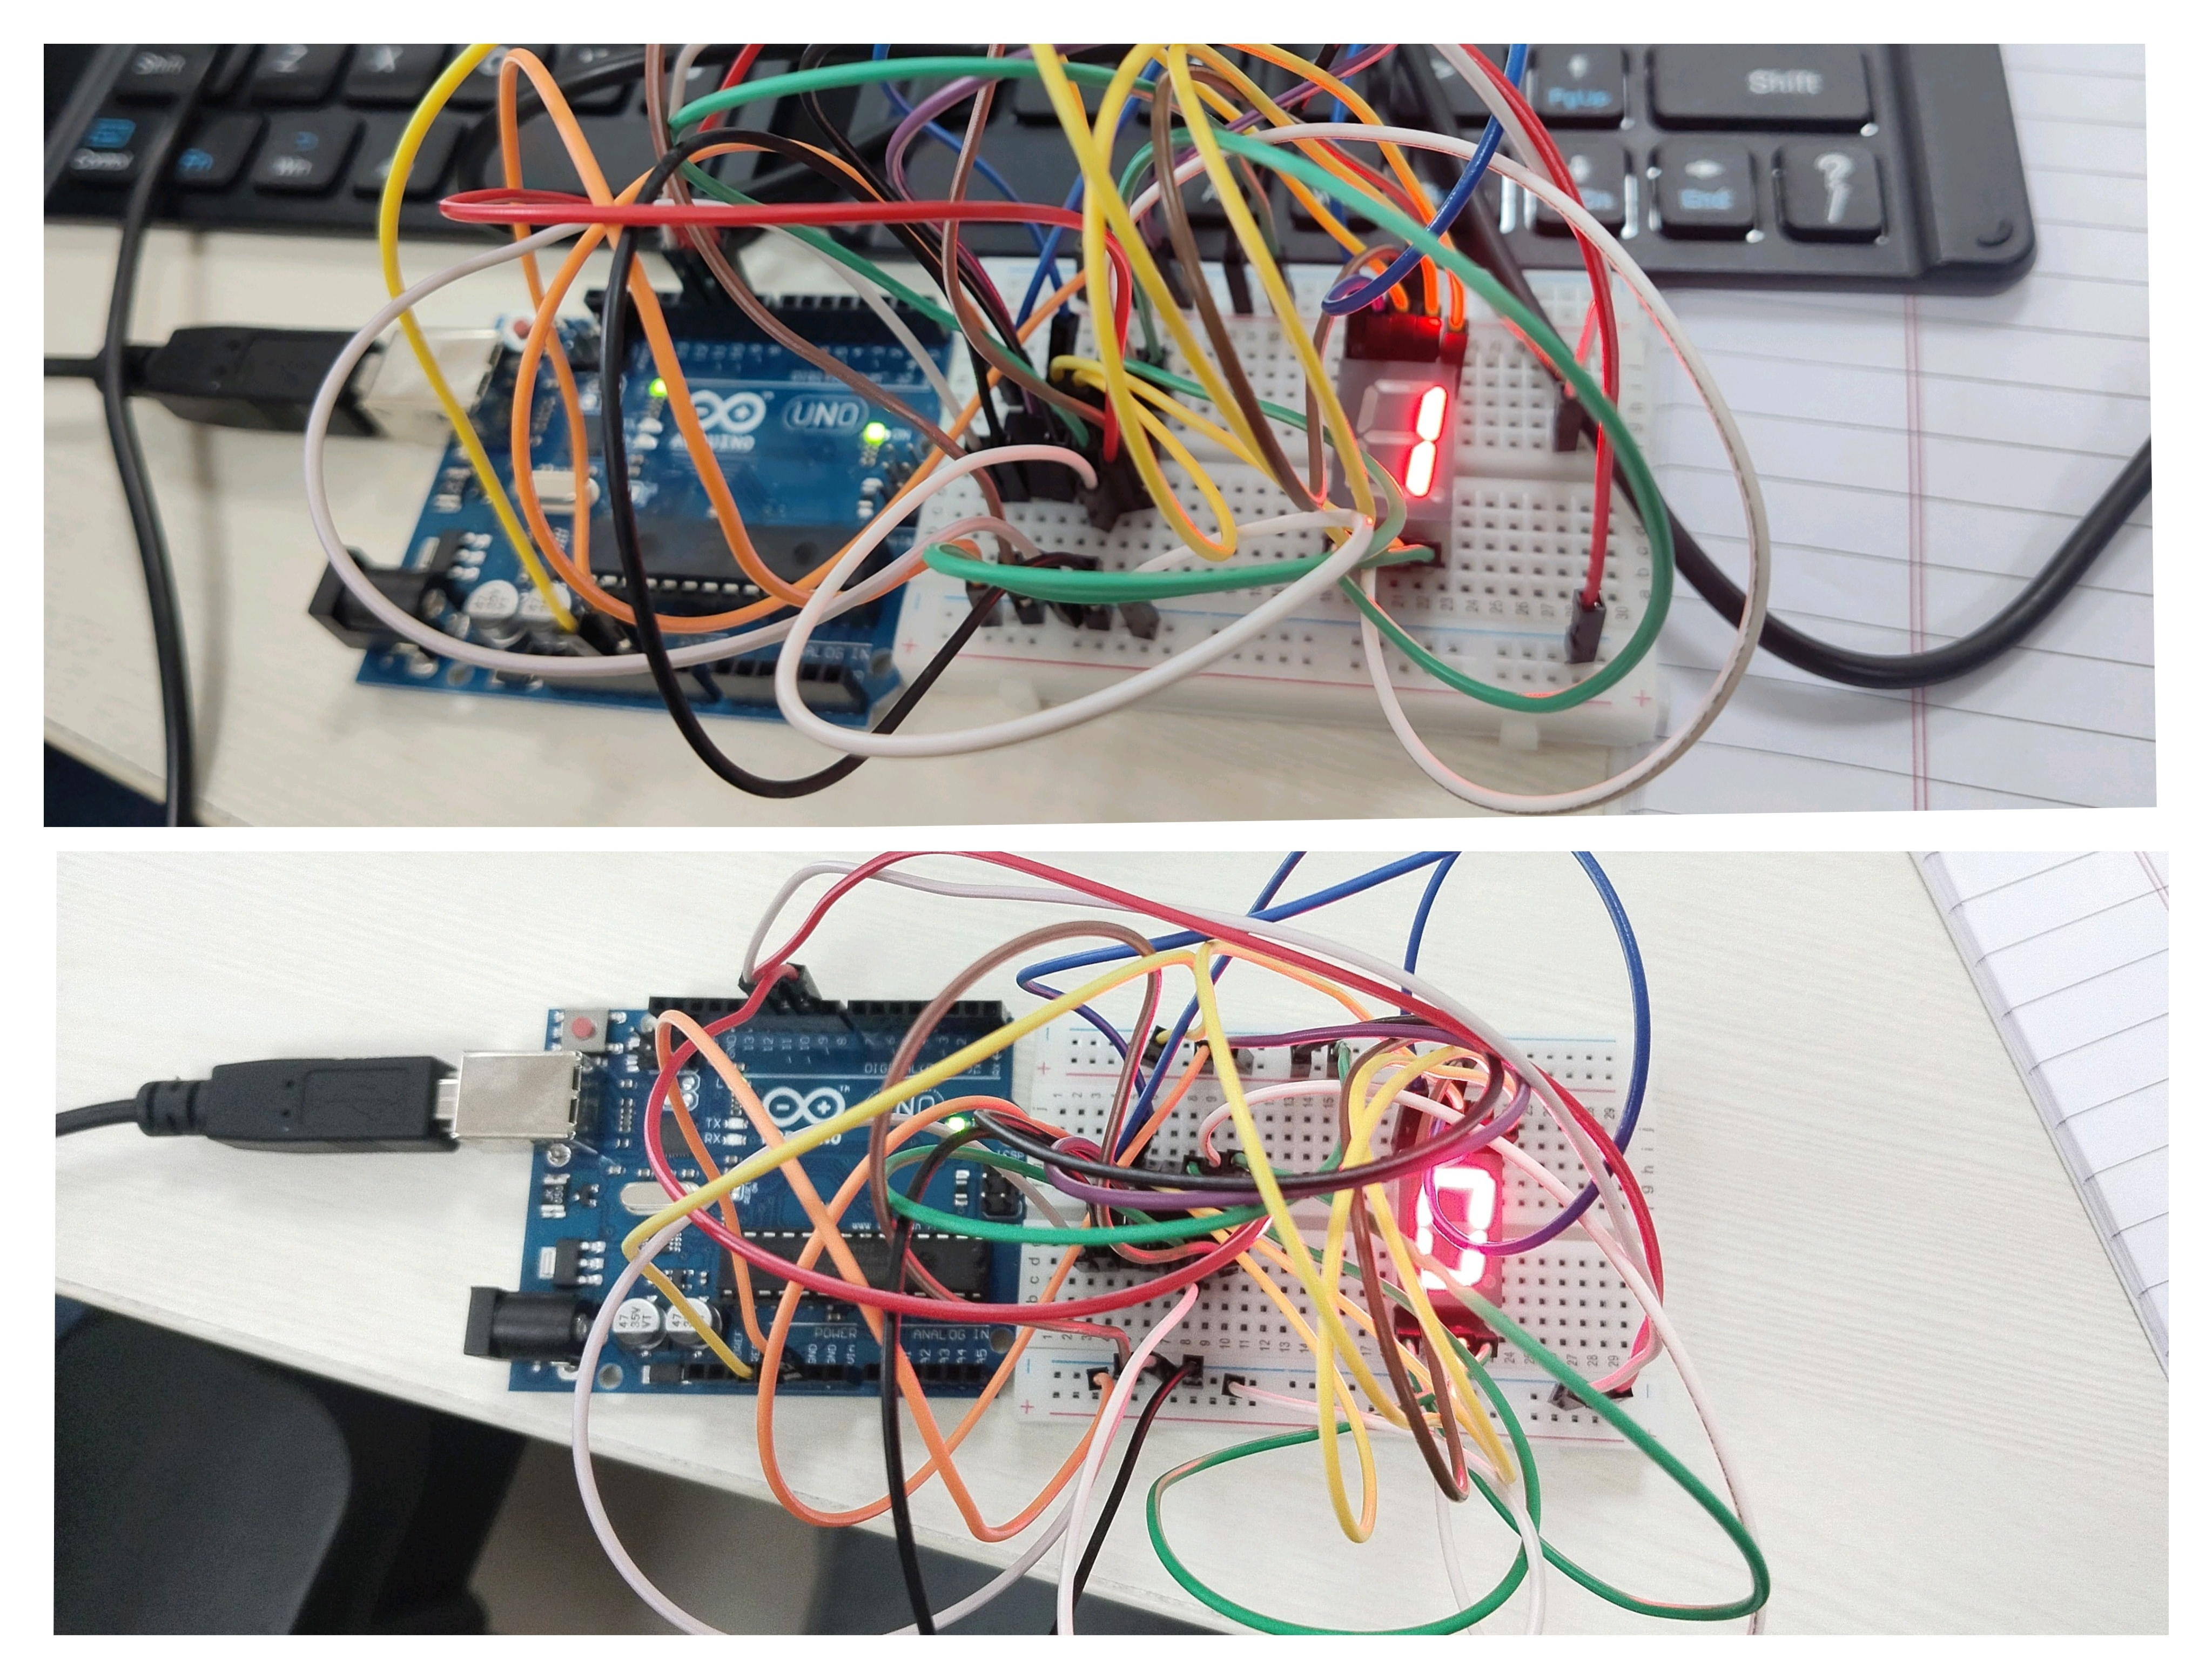
\includegraphics[width=0.8\textwidth]{IMG_20260219_104242.jpg}
\end{center}

\section*{Conclusion}

The given NAND gate circuit realizes the XOR function.

Both theoretical truth table and hardware implementation confirm:

$Z = X \oplus Y$

Hence, the correct answer is \textbf{XOR}.

\end{document}
